% Chapter Template

\chapter{Inferrable Languages} % Main chapter title

\label{ChapterX} % Change X to a consecutive number; for referencing this chapter elsewhere, use \ref{ChapterX}

%----------------------------------------------------------------------------------------
%	SECTION 1
%----------------------------------------------------------------------------------------

\section{Introduction}

The concept of statistics and blackboxes has been drawn out extensively in theories and applications for decades but what of languages and knowing what word can be used to generate the next series of words? Everyone guesses what words can come out of someone talking given enough experience. In this article, the idea of inferrable languages is presented which are languages that allow the next series of words in the sequence to be inferred given enough samples in the sequence.


\section{Applying The Fibonnaci Decider}

Given the definition of the Fibonacci decider and a Lindenmayer system, insight can be derived from to that there exists the commutative and non-commutative properties of the operations. Let the Fibonacci decider for $x_1$, $y_1$, $z_1$ have a determinant equivalent to the identity, -1, then the Fibonacci decider for $x_2$, $y_2$, $z_2$ have a determinant inverse to the identity, 1. The decision functions represented on the six variables is shown below.

$\\ $

$\textbf{Decider}$ for $x_1$, $y_1$, $z_1$

$-x_1 = y_1 - z_1$

$y_1 = -x_1 - z_1$

$-z_1 = x_1 - y_1$

$\\ $

$\textbf{Decider}$ for $x_2, y_2, z_2$

$x_2 = y_2 - z_2$

$-y_2 = x_2 - z_2$

$z_2 = x_2 - y_2$

$\\ $

The Fibonacci decider is a six variable machine on $x_1$, $y_1$, $z_1$, $x_2$, $y_2$, and $z_2$ that decides if the six words are consecutive to each other so that it can completely infer the morphisms of the variables on the sequence.

$\\ $

$\textbf{Fibonacci Decider}$

$x_1 = -y_1 +z_2 - x_2 + y_2 - z_1$

$-y_1 = z_2 - x_2 + y_2 - z_1 + x_1$

$z_2 = -x_2 + y_2 - z_1 + x_1 - y_1$

$-x_2 = y_2 - z_1 + x_1 - y_1 + z2$

$y_2 = -z_1 + x_1 - y_1 + z_2 - x_2$

$-z_1 = x_1 - y_1 + z_2 - x_2 + y_2$

$\\ $

With the Fibonacci decider constructed, apply this concept with a Lindenmayer system. Lindenmayer systems are structures that were originally developed by Aristid Lindenmayer to describe how plants grow. They are simple systems that can be used to model generative concepts. Mathematically speaking, a Lindenmayer system is a deterministic, context-free grammar (shorthand name is D0L systems) defined below.

$\\ $

$\textbf{Lindenmayer System}$

L is the definition of the D0L System

$L = (V,\omega,P)$

$V$ are the characters in the language called the alphabet

$\omega$ is the starting string called the start

$P$ are the production rules in the language called the rules
$\\ $


$\\ $
$\textit{Example 3.2.1}$. As an example the Fibonacci sequence is defined as the sequence below.

$\textit{alphabet}$. $= \{a,b\}$

$\textit{rules}$. $= \{a \Rightarrow ab, b \Rightarrow a\}$

$\textit{start}$. $= b$

$\\ $

With the Fibonacci sequence defined as a Lindenmayer system, the rest of the chapter explains the relation with deciding if a sequence is a Fibonacci sequence and its decomposition to form a language that decides if it is inferrability.

\section{Fibonacci DOL Decider Left Hand Side}

Representing the left hand side of the Fibonacci sequence as a D0L system alphabet requires a alphabet, rules, and a starting state. The left hand side are the two deciders that are composed to form the decider on $x_1 y_1 z_1$ and $x_2 y_2 z_2$. The first six sequences of that form Fibonacci sequence is shown below.

$\\ $

$\textit{Example 3.3.1}$.

$a\ b\ ab\ bab\ abbab\ bababbab$

$\\ $

An important function with sequences and, in particular, words is the length function. Algorithms and functions that operate on words either programmatically or mathematically rely on taking their length. The following example takes the $\textit{example 3.3.1}$ and lists their length.

$\\ $
$\textit{Example 3.3.2}$.

$1\ 1\ 2\ 3\ 5\ 8\ 13\ 21$

$\\ $

A general relationship is found using the value of the length with the Fibonacci sequence and even more generally, is the concept called dynamic programming. The relationship for the sequence specifically is defined as the equation below.

$\\ $
$\textit{Example 3.3.3}$.

$T_n = T_{n-1} + T_{n-2}$

$\\ $

Here, $T_n$ is the current index of the sequence and $T_{n-1}$ and $T_{n-2}$. In the previous chapter, generators are constructed with three variables and on a more general term, it is called the recurrence relation. The Fibonacci decider is not operating on the length specifically but the entirety of its detail which means it operates on the characters of the words in the sequences which will be described in more detail later on. 

$\\ $

$\textit{Example 3.3.4}$. An example of the Fibonacci decider on variables $x_1$, $y_1$, and $z_1$.

$\textbf{Decider}$ for $x_1, y_1, z_1$

$-x_1 = y_1 - z_1$

$-y_1 = -z_1 + x_1$

$z_1 = x_1 + y_1$

$\\ $

$\textit{Example 3.3.5}$. An example of the Fibonacci decider on variables $x_2$, $y_2$, and $z_2$.

$\textbf{Decider}$ for $x_2, y_2, z_2$

$x_2 = y_2 + z_2$

$-y_2 = z_2 - x_2$

$-z_2 = - x_2 + y_2$

$\\ $

In this next example the variables with values from the Fibonacci D0L system is the set such that the conjugation is seen. A conjugation is one such that given a cyclic language and u,v such that they are words in the language, uv and vu are in the language. An example of this is seen where moving the relation of the head variable from third sequence, $z_1$, to the six sequence, $x_2$, below.

$\\ $

$\textit{Example 3.3.6}$. Setting the variables with values from the Fibonacci D0L system.

$x_1 = a$

$y_1 = b$

$z_1 = ab$

$y_2 = bab$

$z_2 = abbab$

$x_2 = bababbab$

$\\ $

$\textit{Example 3.3.7}$. Setting the variables of the decider with values in them and their corresponding column vectors. Here, the negative operation is the inverse operation such that given x,y in the alphabet, $-xy = (xy)^{-1} = y^{-1}x^{-1}$. 

$\\ $

$\textbf{Decider}$ for $x_1, y_1, z_1$

$\\ $

$\textit{\textbf{-x\textsubscript{1} = y\textsubscript{1} - z\textsubscript{1}}}$

$\textit{\textbf{-a = b - ab}}$

$-a + ab = b$

$-b - a = -ab$

$\\ $

$\textbf{-y\textsubscript{1} = -z\textsubscript{1} - x\textsubscript{1}}$

$\textbf{-b = -ab + a}$

ab - b = a

-b -a = -ab

$\\ $

$\textbf{z\textsubscript{1} = x\textsubscript{1}  + y\textsubscript{1}}$

$\textbf{ab = a + b}$

-a + ab = b

ab - b = a

$\\ $

$\textbf{Decider}$ for $x_2, y_2, z_2$

$\\ $

$\textbf{x\textsubscript{2} = y\textsubscript{2} + z\textsubscript{2}}$

$bababbab = bab + abbab$

$bababbab - abbab = bab$

$-bab + bababbab = abbab$

$\\ $

$\textbf{-y\textsubscript{2} = z\textsubscript{2} - x\textsubscript{2}}$

-bab = abbab - bababbab

-abbab - bab = -bababbab

-bab + bababbab = abbab

$\\ $

$\textbf{-z\textsubscript{2} = -x\textsubscript{2} + y\textsubscript{2}}$

-abbab = -bababbab + bab

bababbab - abbab = bab

-abbab - bab = -bababbab

$\\ $

In the next example, generalized equations are elaborated to show the relationship between the each semi-group in the Fibonacci sequence.

$\\ $

$\textit{3.3.8}$. Generalized equations for $x_1$, $y_1$, and $z_1$ as it morphs to general variables $a$, $b$, and $c$, respectively.

$\\ $

$\textit{\textbf{-a = b - c}}$

$-a + c = b$

$-b - a = -c$

$\\ $

$\textbf{-b = -c + a}$

c - b = a

-b - a = -c

$\\ $

$\textbf{c = a + b}$

-a + c = b

c - b = a

$\\ $

Generalized equations for $x_2$, $y_2$, $z_2$ as it maps to $a$, $b$, and $c$, respectively.

$\\ $

$\textbf{-b = c - a}$

-c - b = -a

-b + a = c

$\\ $

$\textbf{-c = -a + b}$

a - c = b

-c - b = -a

$\\ $

$\textit{\textbf{a = b + c}}$

$a - c = b$

$-b + a = c$

$\\ $

It can be noted that each semi-group, $x_1 y_1 z_1$ and $y_2 z_2 x_2$, revolves clockwise independently from each other.

\section{Fibonacci DOL Decider Right Hand Side}

$\textbf{Fibonacci Decider}$

$x_1 = -y_1 + z_2 - x_2 + y_2 - z_1$

$-y_1 = z_2 - x_2 + y_2 - z_1 + x_1$

$z_2 = -x_2 + y_2 - z_1 + x_1 - y_1$

$-x_2 = y_2 - z_1 + x_1 - y_1 + z_2$

$y_2 = -z_1 + x_1 - y_1 + z_2 - x_2$

$-z_1 = x_1 - y_1 + z_2 - x_2 + y_2$

$\\ $

$
\begin{matrix}
 \textbf{a = -b + abbab - bababbab + bab - ab}\\
a + ab - ab - a + bab = -abaab \\
bababbab + abaab + ab - a + bab = b \\
bababbab + abaab - b - a + bab = -ab \\
bababbab + abaab - b + ab + bab = a \\
bababbab + abaab - b + ab - a = -bab \\
\end{matrix}
$

$\\ $

$
\begin{matrix}
 \textbf{-abaab = b - ab + a -bab + bababbab}\\
-abaab + ab - a + bab - bababbab = b \\
-abaab - b - a + bab - bababbab = -ab \\
-abaab - b + ab + bab - bababbab = a\\
-abaab - b + ab - a - bababbab = -bab\\
-abaab - b + ab - a + bab = bababbab \\
\end{matrix}
$

$\\ $

$
\begin{matrix}
 \textbf{b = -ab + a - aba + abaababa - abaab}\\
b - a + aba - abaababa + abaab = -ab \\
b + ab + aba - abaababa + abaab = a \\
b + ab + aba - abaababa + abaab = -aba\\
b - ab + a -aba + abaab = abaababa\\
b - ab - a + aba - abaababa = -abaab \\
\end{matrix}
$

$\\ $

$
\begin{matrix}
 \textbf{-ab = a - aba + abaababa - abaab + b}\\
- ab + aba - abaababa + abaab - b = a \\
- ab - a - abaababa + abaab -b = - aba \\
- ab - a + aba + abaab - b = abaababa\\
- ab -a + aba - abaababa - b = -abaab\\
-ab - a + aba -  abaababa + abaab = b\\
\end{matrix}
$

$\\ $

$
\begin{matrix}
 \textbf{a = aba + abaababa - abaab + b - ab}\\
a + abaababa - abaab + b - ab = aba \\
a - aba - abaab + b - ab = -abaababa \\
a - aba + abaababa + b - ab = abaab\\
a - aba + abaababa - abaab - ab = -b\\
a - aba + abaababa - abaab + b = ab\\
\end{matrix}
$

$\\ $

$
\begin{matrix}
 \textbf{-aba = abaababa - abaab + b - ab + a}\\
- aba + abaab - b + ab - a = abaababa \\
-aba - abaababa - b + ab + a = -abaab \\
-aba - abaababa + abaab + ab - a = b\\
-aba - abaababa + abaab - b - a = -ab\\
-aba - abaababa + abaab - b + ab = a\\
\end{matrix}
$

\section{The Law of Commutativity and Noncommutativity}

The law of commutativity and the law of noncommutativity combined gives the law of commutativity and noncommutativity

$\\ $
 
The Law of Commutativity

a + b = b + a

ex. 8 + 5 = 5 + 8

$\\ $

The Law of Noncommutativity

a+ b != b + a

ex. 8 - 5 != 5 - 8

$\\ $

Each equation in the example on the left has permutations.

From this example, it can be implied that for every variable, n, in an equation there is $n^2$ permutations in the sequence.

The first equation is bold and italicized in the set to make a decider.



$
\begin{matrix}
 \textit{\textbf{a = b + c}} & \textbf{b = a - c} & \textbf{-c = a - b}\\
 b = a - c & b - a = -c & -c + b = a\\
 -c = a - b & b + c = a & -c - a = -b
\end{matrix}
$

\section{Operations}

Operations for the right hand side (RHS) versus the left hand side (LHS) represents different operations of the string in different scenarios.

$\\ $

RHS Evaluation

Right to Left

+ Remove from the back

- Add to the front

abaababa = - abaab + b - ab + a -aba

abaababa = - abaab + b - ab -ab

abaababa = - abaab + b - abab

abaababa = - abaab - aba

abaababa = - abaababa

$\\ $

LHS Evaluation

Left to Right

+ Remove at the front

- Add to the back

abaababa + abaab - b + ab - a = -aba

aba - b + ab - a = -aba

abab + ab - a = -aba

ab - a = -aba

aba = -aba

$\\ $

$\textit{Proposition.}$The characteristic series of a rational cyclic language is a Z-linear combination of characters of finite deterministic automata.

$\\ $

\section{Definition Of Support}

A support is defined as the following:

A* is a word

S is the function

Image by S of a word w is denoted by (S,w) and is the coefficient of w in S

Support(S) = {w in A* such that (S,w) != 0}

$\\ $

Now we take deciders of a monomial and the picking function to redefine the support of a noncommutative rational language

R is the rational numbers where x in R = a/b

such that a,b is in integers and b $\neq$ 0

Q is the quotient space represented in topology such that A/~ where are sets and ~ is the divisions of A

R-rational is the representation of R as the polynomial function

Q-rational is the representation of Q as a polynomial

\section{Rationals Of Picking Function}

Support of the Fibonacci Picking Function of the deciders of a monomial.

Q-rational-deciders are the possible monomial deciders of Q-rational-string. Use the picking function, PF, to choose one decision function in Q-rational-deciders, we see a mapping from Q-rational => R-rational.

\begin{figure}[H]
  \centering
  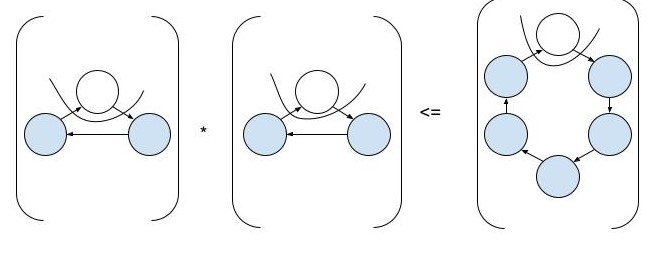
\includegraphics[width=\linewidth]{0219Rationals.jpg}
  \caption{Q rational image of the q rational string, $x^3/3$, $x^3/3$, and $X^6/x$.}
  \label{fig:0219Rationals}
\end{figure}

Deciders for $x^3/x$ has 9 possible configurations, or, in algebraic terms, permutations, and $x^6/x$ has 36 possible configurations. This equates to R rational for $x^3/x$ being $1/9$ and $x^6/x$ being $1/36$.

This implies the existence of the map between Q rational to R rational.

\section{Support Of Picking Function}

The support of an inferrable language is now defined to be:

$\\ $

Dupport of PF of Q-rational-deciders = support(PF(Q-rational-deciders))

$\\ $

Decider in Q-rational-deciders such that decider is unique $\equiv$ Determinant of a configuration of a decider != 0

\section{Law Of Strings}

$
\begin{matrix}
 \textit{\textbf{a = b + c}} & \textbf{b = a - c} & \textbf{-c = a - b}\\
 b = a - c & b - a = -c & -c + b = a\\
 -c = a - b & b + c = a & -c - a = -b
\end{matrix}
$

$\\ $

$
\begin{matrix}
 (\textit{\textbf{LHS}} = RHS) \neq (\textit{\textbf{RHS}} & \textbf{LHS})\\
 (\textit{\textbf{LHS}} = \textbf{RHS}) = (\textit{\textbf{RHS}} & \textit{LHS})\\
\end{matrix}
$

$\\ $

Condense the above to get a generalization.

$\\ $

$
\begin{matrix}
a = -a & -a = a\\
a \neq -a & -a \neq a
\end{matrix}
$

$\\ $

This is operating on variables, strings, and representations of it.

\section{Commutativity Of Addition}

$
\begin{matrix}
a + b = b - a & b - a = a + b\\
b + a = -a + b & - a + b = b + a\\
\\
a + b \neq b - a & -a + b \neq b + a\\
b + a \neq -a + b & b - a \neq a + b
\end{matrix}
$

$\\ $

Take the length function, length(s) $\equiv$ l(s), and apply to the '=' addition operations and see it's equivalence. Set b to a and reversal is accomplished.

$\\ $

$
\begin{matrix}
len(a) + len(b) = len(b)+ len(-a) \equiv 11 = 11 & len(b) + len(-a) = len(a) + len(b) \equiv 11 = 11\\
len(b) + len(a) = len(-a) + len(b) \equiv 11 = 11 & len(-a) + len(b) = len(b) + len(a) \equiv 11 = 11\\
\\
a + b \neq b - a \equiv 11 \neq 10 & -a + b \neq b + a \equiv 01 \neq 11\\
b + a \neq -a + b \equiv 11 \neq 01 & b - a \neq a + b \equiv 10 \neq 11
\end{matrix}
$

\section{Commutativity Of Multiplication}

$
\begin{matrix}
a * b = b * -a & b * -a = a * b\\
b * a = -a * b & - a * b = b * a\\
\\
a * b \neq b * -a & -a * b \neq b * a\\
b * a \neq -a * b & b * -a \neq a * b
\end{matrix}
$

\section{Additive Identity}

$
\begin{matrix}
a = -a\ for\ any\ a\ is\ equal\ to\ -a & -a\ =\ a\ where\ a\ and\ -a\ is\ 1\\
a \neq -a\ where\ a\ is\ 1\ and\ -a\ is\ 0 & -a \neq a\ where\ a\ is\ 1\ and\ -a\ is\ 0
\end{matrix}
$

The LHS and RHS are equations that test whether or not they are true or false, or in terms of computational complexity theory, it is satisfiable.
10 = 10 evaluates to true or 1.
01 != 10 evaluates to true or 1 too.

\section{Multiplicative Identity}

$
\begin{matrix}
a = -a\ where\ a\ and\ -a\ are\ 1 \equiv\ a\ represented\ as\ monomial\ decider\ loops\ once\\
a \neq -a\ where\ a\ is\ 1\ and\ -a\ is\ 0 \equiv a\ represented\ as\ a\ monomial\ decider\ loops\ once
\end{matrix}
$

\section{Additive Inverse}

The Additive Inverse

$\\ $

General Equivalence

$
\begin{matrix}
a + l = -a + r \equiv 10 = 10 & -a + r = a + l \equiv 10 = 10\\
l + a = r - a \equiv 10 = 10 & r - a = l + a \equiv 10 = 10\\
\end{matrix}
$

$\\ $

Commutativity under Equivalence

$
\begin{matrix}
a + l = r - a \equiv 10 = 10 & -a + r = l + a \equiv 10 = 10\\
l + a = -a + r \equiv 10 = 10 & r - a = a + l \equiv 10 = 10\\
\end{matrix}
$


$\\ $

General Reversal

$
\begin{matrix}
a + l \neq -a + r \equiv 10 = 01 & -a + r \neq a +l \equiv 01 = 10\\
l + a \neq r - a \equiv 10 = 01 & r - a \neq l + a \equiv 01 = 10\\
\end{matrix}
$

$\\ $

Commutativity under reversal

$
\begin{matrix}
a + l \neq r - a \equiv 10 = 01 & -a + r \neq l + a \equiv 01 = 10\\
l + a \neq - a + r \equiv 10 = 01 & r - a \neq a + l \equiv 01 = 10\\
\end{matrix}
$

$\\ $

\begin{figure}[H]
  \centering
  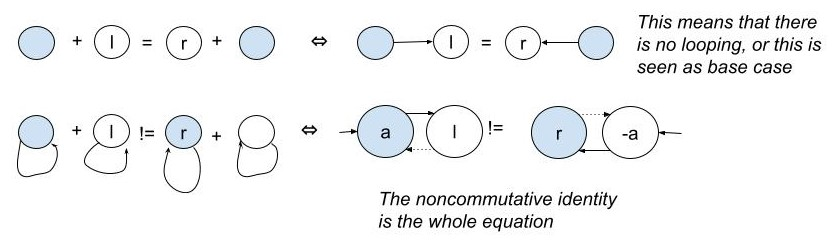
\includegraphics[width=\linewidth]{0220AdditiveInverse.jpg}
  \caption{Additive inverse direction.}
  \label{fig:0220AdditiveInverse}
\end{figure}


\section{Multiplicative Inverse}

Given a monomial such that it represents a monomial in a polynomial, if we loop around once, we see the identity path.

$\\ $

General Equivalence

$
\begin{matrix}
a * L = -a * R \equiv 10 = 10 & -a * R = a + L \equiv 10 = 10\\
L * a = R * - a \equiv 10 = 10 & R * -a = L*a \equiv 10 = 10\\
\end{matrix}
$

$\\ $

Commutativity under Equivalence

$
\begin{matrix}
a * L = R * -a \equiv 10 = 10 & -a * R = L * a \equiv 10 = 10\\
L * a = -a * R \equiv 10 = 10 & R * -a = a * L \equiv 10 = 10\\
\end{matrix}
$


$\\ $

General Reversal

$
\begin{matrix}
a*L \neq -a*R \equiv 10 = 01 & -a*R \neq a*L \equiv 01 = 10\\
L*a \neq R*-a \equiv 10 = 01 & R*-a \neq L*a \equiv 01 = 10\\
\end{matrix}
$

$\\ $

Commutative under Reversal

$
\begin{matrix}
a*L \neq R*-a \equiv 10 = 01 & -a*R\neq L*a \equiv 01 = 10\\
L*a \neq - a*R \equiv 10 = 01 & R*-a \neq a*L \equiv 01 = 10\\
\end{matrix}
$

$\\ $

\begin{figure}[H]
  \centering
  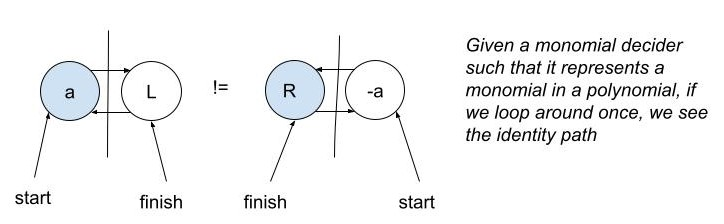
\includegraphics[width=\linewidth]{0221MultiplicativeInverse.jpg}
  \caption{Multiplicative inverse direction.}
  \label{fig:0221MultiplicativeInverse}
\end{figure}

\section{Generalized Operations}

The set of images that describes the operations on monomials can be put together to find a 2x2 matrix that describes them using the laws provided.


\begin{figure}[H]
  \centering
  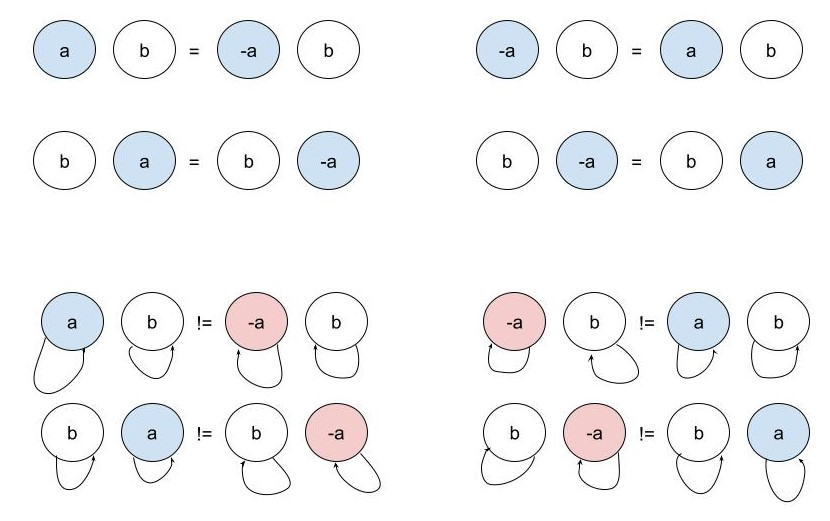
\includegraphics[width=\linewidth]{0222Operations.jpg}
  \caption{Generalized operations.}
  \label{fig:0222Operations}
\end{figure}

\section{Generalized Communativity}

For showing commutativity, have the following images to represent addition and multiplication. Fibonacci sequences are seen to be non-commutative if they are seen in this regards.

\begin{figure}[H]
  \centering
  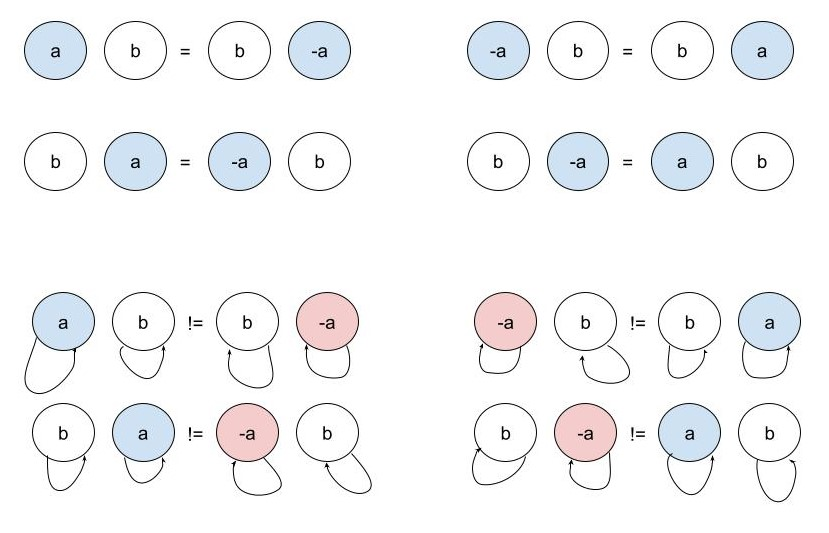
\includegraphics[width=\linewidth]{0223Commutativity.jpg}
  \caption{Communativity.}
  \label{fig:0223Commutativity}
\end{figure}

\section{Associativity Of Addition}

Associativity of addition is defined as:

a + (b + c) = (a + b) + c

\begin{figure}[H]
  \centering
  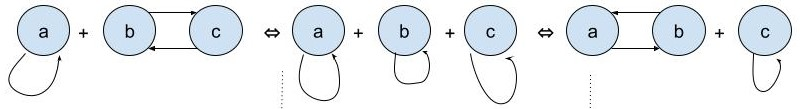
\includegraphics[width=\linewidth]{0224AssociativityOfAddition.jpg}
  \caption{Associativity of addition.}
  \label{fig:0224AssociativityOfAddition}
\end{figure}

$\\ $

a + bc

$\\ $

$
\begin{matrix}
a = -a & -a = a \\
a \neq -a & -a \neq a\\
\end{matrix}
$

$\\ $

$
\begin{matrix}
b + c = -b + c & -b + c = b + c\\
c + b\neq -c+b & -c+b \neq c + b\\\
\\
c + b= c+b & -b + c = c + b\\
c + b\neq -c+b & -c+b \neq c + b\\
\\
b + c = c-b & c-b = b + c\\
b + c\neq c-b & c-b \neq b+ c\\
\\
c + b = b + c & -c+b = b + c\\
c + b \neq b-c & -c+b \neq b + c\\
\end{matrix}
$

$\\ $

a + b + c

$\\ $

$
\begin{matrix}
a = -a & -a = a \\
a \neq -a & -a \neq a\\
\end{matrix}
$

$\\ $

$
\begin{matrix}
b = -b & -b = b \\
b \neq -b & -b \neq b\\
\end{matrix}
$

$\\ $

$
\begin{matrix}
c = -c & -c = c \\
c \neq -c & -c \neq c\\
\end{matrix}
$

$\\ $

ab + c

$\\ $

$
\begin{matrix}
a + b = -a + b & -a + b = a + b\\
b + a\neq -b+a & -b+a \neq b + a\\\
\\
b + a= b+a & -a + b = b + a\\
b + a\neq -b+a & -b+a \neq b + a\\
\\
a + b = b-a & b-a = a + b\\
a + b\neq b-a & b-a \neq a+ b\\
\\
b + a = a + b & -b+a = a + b\\
b + a \neq a-b & -b+a \neq a + b\\
\end{matrix}
$

$\\ $

$
\begin{matrix}
c = -c & -c = c \\
c \neq -c & -c \neq c\\
\end{matrix}
$


\section{Associativity Of Multiplication}

Associativity of multiplication is defined as:

a * (b*c) = (a*b)*c

$\\ $

\begin{figure}[H]
  \centering
  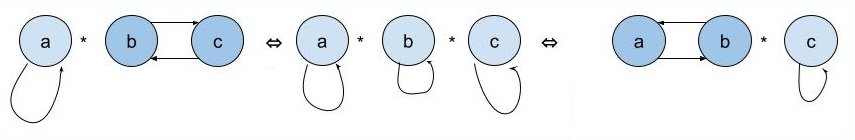
\includegraphics[width=\linewidth]{0225AssociativityOfMultiplication.jpg}
  \caption{Associativity of multiplication.}
  \label{fig:0225AssociativityOfMultiplication}
\end{figure}

$\\ $

a + bc

$\\ $

$
\begin{matrix}
a = -a & -a = a \\
a \neq -a & -a \neq a\\
\end{matrix}
$

$\\ $

$
\begin{matrix}
b * c = -b * c & -b * c = b * c\\
c * b\neq -c*b & -c*b \neq c * b\\\
\\
c * b= c*b & -b * c = c * b\\
c * b\neq -c*b & -c*b \neq c * b\\
\\
b * c = c-b & c-b = b * c\\
b * c\neq c-b & c-b \neq b* c\\
\\
c * b = b * c & -c*b = b * c\\
c * b \neq b-c & -c*b \neq b * c\\
\end{matrix}
$

$\\ $

a + b + c

$\\ $

$
\begin{matrix}
a = -a & -a = a \\
a \neq -a & -a \neq a\\
\end{matrix}
$

$\\ $

$
\begin{matrix}
b = -b & -b = b \\
b \neq -b & -b \neq b\\
\end{matrix}
$

$\\ $

$
\begin{matrix}
c = -c & -c = c \\
c \neq -c & -c \neq c\\
\end{matrix}
$

$\\ $

ab + c

$\\ $

$
\begin{matrix}
a * b = -a * b & -a * b = a * b\\
b * a\neq -b*a & -b*a \neq b * a\\\
\\
b * a= b*a & -a * b = b * a\\
b * a\neq -b*a & -b*a \neq b * a\\
\\
a * b = b-a & b-a = a * b\\
a * b\neq b-a & b-a \neq a* b\\
\\
b * a = a * b & -b*a = a * b\\
b * a \neq a-b & -b*a \neq a * b\\
\end{matrix}
$

$\\ $

$
\begin{matrix}
c = -c & -c = c \\
c \neq -c & -c \neq c\\
\end{matrix}
$

\section{Distibutivity}

Distributivity is defined as:

$\textbf{a*(b+c) = a*b + a*c}$.

\begin{figure}[H]
  \centering
  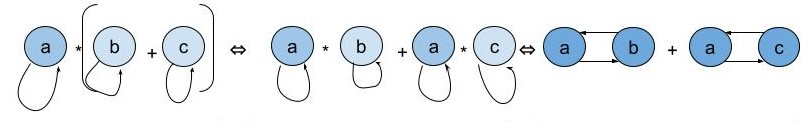
\includegraphics[width=\linewidth]{0226Distributivity.jpg}
  \caption{Associativity of multiplication.}
  \label{fig:0226Distributivity}
\end{figure}

$\\ $

$\textbf{a + b + c}$

$\\ $

$
\begin{matrix}
a = -a & -a = a \\
a \neq -a & -a \neq a\\
\end{matrix}
$

$\\ $

$
\begin{matrix}
b = -b & -b = b \\
b \neq -b & -b \neq b\\
\end{matrix}
$

$\\ $

$
\begin{matrix}
c = -c & -c = c \\
c \neq -c & -c \neq c\\
\end{matrix}
$

$\\ $

$\textbf{a b + a c}$

$\\ $

$
\begin{matrix}
a = -a & -a = a \\
a \neq -a & -a \neq a\\
\end{matrix}
$

$\\ $

$
\begin{matrix}
b = -b & -b = b \\
b \neq -b & -b \neq b\\
\end{matrix}
$

$\\ $

$
\begin{matrix}
a = -a & -a = a \\
a \neq -a & -a \neq a\\
\end{matrix}
$

$\\ $

$
\begin{matrix}
c = -c & -c = c \\
c \neq -c & -c \neq c\\
\end{matrix}
$

$\\ $

$\textbf{a b + a c}$

$\\ $

$
\begin{matrix}
a * b = -a * b & -a * b = a * b\\
a * b \neq -a * b & -a * b \neq a * b\\
\\
b * a = -b*a & -b*a = b * a\\
b * a\neq -b*a & -b*a \neq b * a\\
\\
\\
a * b = b-a & b-a = a * b\\
a * b \neq b-a & b-a \neq a * b\\
\\
b * a = a * -b & -b*a = a * b\\
b * a \neq a * -b & -b*a \neq a * b\\
\end{matrix}
$

$\\ $

$
\begin{matrix}
a * c = -a * c & -a * c = a * c\\
a * c \neq -a * c & -a * c \neq a * c\\
\\
c * a = -c*a & -c*a = c * a\\
c * a\neq -c*a & -c*a \neq c * a\\
\\
\\
a * c = c-a & c-a = a * c\\
a * c \neq c-a & c-a \neq a * c\\
\\
c * a = a * -c & -c*a = a * c\\
c * a \neq a * -c & -c*a \neq a * c\\
\end{matrix}
$

\section{Field}

These rules result in a field defined by Wolfram.

$\\ $

$
\begin{matrix}
Axioms & Addition & Multiplication\\
Commutativity & a+b = b+a & a*b = b*a\\
Identity & a+0 = a = 0+a & a*1 = a = 1*a\\
Inverses & a+(-a)=0=(-a)+a & a*a^-1 = 1 = a^-1*a\ if\ a != 0\\
Associativity & (a+b)+c = a+(b+c) & (a*b)*c = a*(b*c)\\
Distributivity & a*(b+c) = a*b+a*c & (a+b)*c = a*(b+c)
\end{matrix}
$

$\\ $

This field is seen in $\textit{Garg, Gurvits, Oliveira, and Wigderson}$. 